\documentclass[12pt,a4paper]{article}
\usepackage[UTF8]{ctex}
\usepackage{amsmath}
\usepackage{graphicx}
\usepackage{booktabs}
\usepackage{geometry}
\usepackage{siunitx}
\usepackage{ulem}
\usepackage{caption}
\geometry{left=2.5cm,right=2.5cm,top=2.5cm,bottom=2.5cm}
\sisetup{per-mode=symbol}

\title{\Huge{\textbf{\uuline{预\ 习\ 报\ 告}}}}
\author{\uline{少年班学院} \quad 姓名: \uline{李大恕} \quad 学号: \uline{PB24000145}}
\date{\today}

\begin{document}
\maketitle

\section{实验题目}
部分相干光源的空间相干性测量与分析

\section{实验目的}
\begin{enumerate}
    \item 理解部分相干光源的空间相干性及其随横向距离衰减的物理含义。
    \item 掌握利用激光与旋转毛玻璃产生部分相干光的方法。
    \item 熟悉改进迈克尔逊干涉光路中光程差、平面镜倾角和柱透镜反转对干涉图样的影响。
    \item 观察不同毛玻璃状态和位置下干涉条纹区域及条纹对比度的变化，分析部分相干光的空间相干特性。
\end{enumerate}

\section{实验原理}
\subsection{部分相干光的空间相干性}
部分相干光的重要特征是光场中不同横向位置之间只具有有限的相干性。两点之间的横向距离越大，其相干程度越弱，因而只有距离较近的光场点之间才能形成较清晰、稳定的干涉条纹。以部分相干的 Collett-Wolf 光源为例，空间相干度 $g(\rho)$ 与两点间距离 $\rho$ 的关系可写为
\begin{equation}
    g(\rho)=\exp\left(-\frac{\rho^2}{2\sigma_g^2}\right),
    \label{eq:coherence}
\end{equation}
其中 $\sigma_g$ 是相干性衰减的特征尺度。当 $\rho$ 超过这一尺度后，相干度迅速减小，干涉条纹的可见度也随之下降。

部分相干光在远距离传输过程中光强分布较为均匀，干涉条纹清晰稳定，同时可以有效降低激光散斑的影响；但其空间相干性会随横向距离快速衰减，因此横向相距较远的两束光难以产生明显干涉。

\subsection{迈克尔逊干涉与条纹对比度}
在迈克尔逊干涉仪中，入射光经分束后形成两束光，两束光分别经平面镜反射后重新叠加。调节两臂的光程差可以改变干涉相位，调节平面镜之间的相对倾角可以得到不同方向和不同间距的干涉条纹。

干涉条纹的清晰程度通常用条纹对比度表示：
\begin{equation}
    V=\frac{I_{\max}-I_{\min}}{I_{\max}+I_{\min}},
    \label{eq:visibility}
\end{equation}
其中 $I_{\max}$ 和 $I_{\min}$ 分别为局部条纹强度的最大值和最小值。对于部分相干光，条纹对比度与两束叠加光之间的相干程度密切相关。当两束光对应的源面点横向间距较小时，互相干性较强，条纹对比度较高；当对应点间距增大时，互相干性降低，条纹逐渐变浅甚至消失。

\subsection{部分相干光源相干性测量光路}
本实验在迈克尔逊干涉光路的基础上进行改造，用激光与旋转毛玻璃组合产生部分相干光源，并在其中一路加入柱透镜，使分束后的某一束光在竖直方向发生反转。实验光路如图~\ref{fig:optical_path} 所示。

\begin{figure}[htbp]
    \centering
    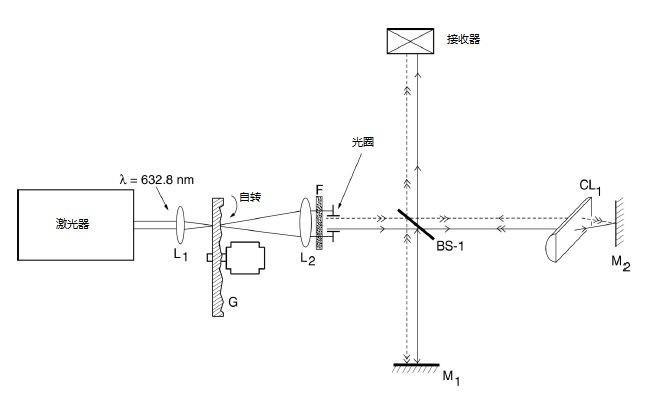
\includegraphics[width=0.72\textwidth]{assets/page2_img2_Image53.jpg}
    \caption{部分相干光空间相干性测量光路}
    \label{fig:optical_path}
\end{figure}

激光经透镜扩束和毛玻璃散射后形成具有有限空间相干尺度的光场，再经光阑、分束器和平面镜构成双光束干涉。由于柱透镜将其中一路光束作竖直方向反转，屏幕或 CCD 上同一位置处叠加的两束光实际对应于源面上一对互为镜像的光场点。两点之间的横向距离随观察位置改变而改变，因此不同区域的条纹对比度不同。靠近相干性较好的重合区域时，条纹较清晰；远离该区域时，两束光对应点的横向间距增大，空间相干性减弱，条纹逐渐消失。

\subsection{毛玻璃状态对干涉图样的影响}
未加入毛玻璃时，入射光近似为普通激光光源，CCD 上可观察到典型的迈克尔逊干涉条纹。加入静止毛玻璃后，光场出现明显散斑，部分区域仍可看到条纹。散斑内的光场具有较好的局部相干性，但不同散斑之间相位关系不稳定。

当毛玻璃旋转并达到一定速度时，毛玻璃表面微小颗粒的切换时间短于 CCD 的曝光时间，CCD 记录到的是多个随机相位散斑场的时间平均结果。无固定相位关系处的光强被平均，相干性较弱的区域条纹被削弱；相干性较好的区域仍保留较明显的干涉条纹，表现为条纹对比度在中间区域较高、两侧较低。

\section{实验仪器}
实验装置如图~\ref{fig:device} 所示，主要元件包括：
\begin{itemize}
    \item 波长为 \SI{532}{\nano\meter} 的半导体激光器；
    \item 焦距为 \SI{15}{\milli\meter} 的凸透镜 L1；
    \item 焦距为 \SI{50}{\milli\meter} 的凸透镜 L2；
    \item 毛玻璃 G 及其步进电机；
    \item 直径可调的光阑 F；
    \item 平面镜 M1、M2；
    \item 焦距为 \SI{2}{\centi\meter} 的水平放置柱透镜 CL1；
    \item 分束器、CCD 成像系统及光学平台。
\end{itemize}

\begin{figure}[htbp]
    \centering
    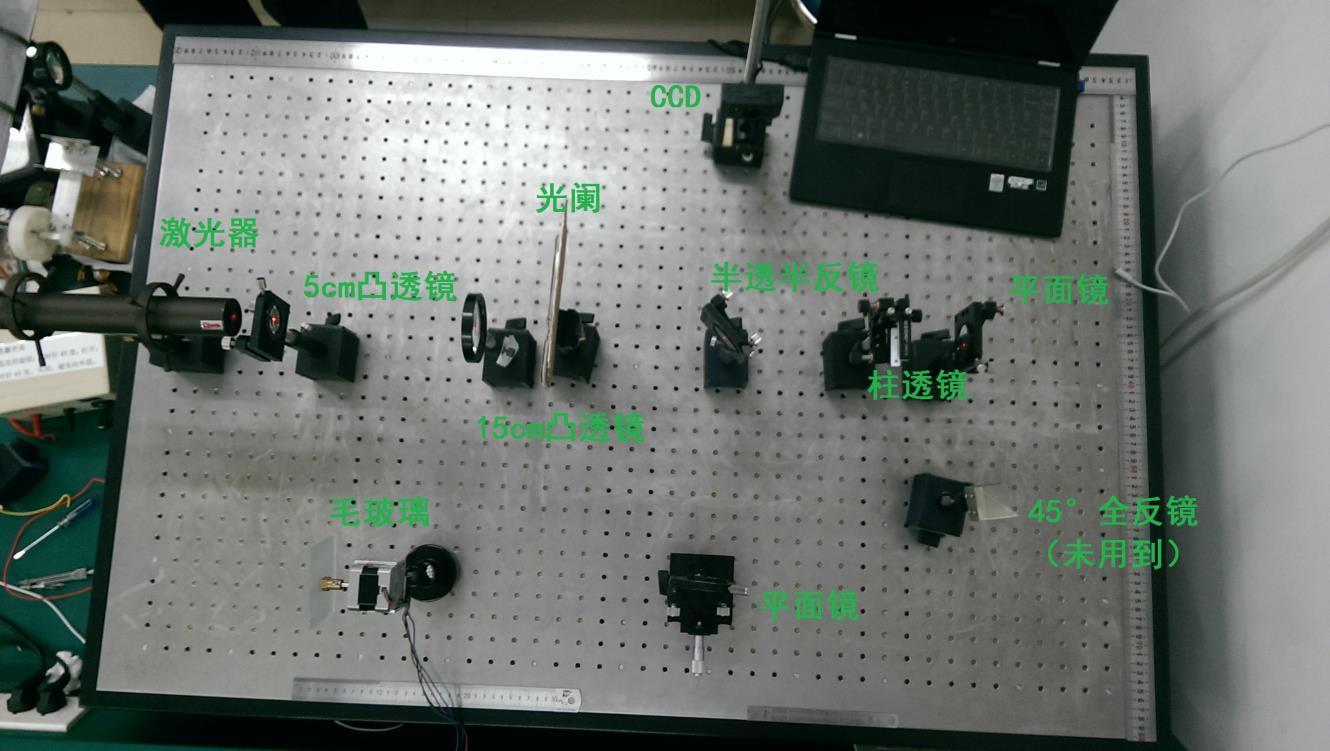
\includegraphics[width=0.82\textwidth]{assets/page3_img1_Image63.jpg}
    \caption{部分相干光空间相干性测量实验装置}
    \label{fig:device}
\end{figure}

\section{实验步骤}
\begin{enumerate}
    \item 按照实验光路安装激光器、透镜、毛玻璃及步进电机、光阑、分束器、平面镜、柱透镜和 CCD，使各光学元件共轴，光轴平行于光学平台。
    \item 调整下方平面镜的位置和倾角，使 CCD 图像上的干涉条纹尽可能粗。此时两分光路近似等光程，两平面镜近似互相垂直。
    \item 继续微调平面镜，使两平面镜在水平或竖直方向存在适当夹角，分别获得竖直、水平或倾斜方向的干涉条纹，并观察条纹间距的变化。
    \item 在未加入毛玻璃的条件下观察普通迈克尔逊干涉图样，记录条纹方向、间距和清晰程度。
    \item 加入静止毛玻璃，观察散斑背景中的干涉条纹，比较其与未加入毛玻璃时的差别。
    \item 启动步进电机使毛玻璃旋转，观察条纹范围和对比度的变化。重点记录条纹是否只在部分区域保留，以及中间区域和两侧区域的条纹清晰程度。
    \item 改变旋转毛玻璃的位置，例如将毛玻璃置于焦点附近或远离焦点处，记录存在明显干涉条纹的区域变化。
    \item 对 CCD 图像中不同位置的条纹强度分布进行分析，可由式~\eqref{eq:visibility} 计算局部条纹对比度，并比较不同毛玻璃状态和位置下空间相干性的变化。
\end{enumerate}

\section{预期现象与分析}
未加入毛玻璃时，干涉图样主要由两臂光程差和平面镜相对倾角决定，条纹分布类似普通迈克尔逊干涉。加入静止毛玻璃后，散斑结构叠加在干涉图样上，局部仍可观察到条纹。毛玻璃旋转后，随机散斑随时间平均，只有空间相干性较强的区域保留较明显条纹；由于柱透镜使其中一路光束发生反转，两个圆形光斑的交叠区域内不同位置对应的源面点间距不同，因此会出现条纹对比度中间较高、两侧较低的现象。

\begin{figure}[htbp]
    \centering
    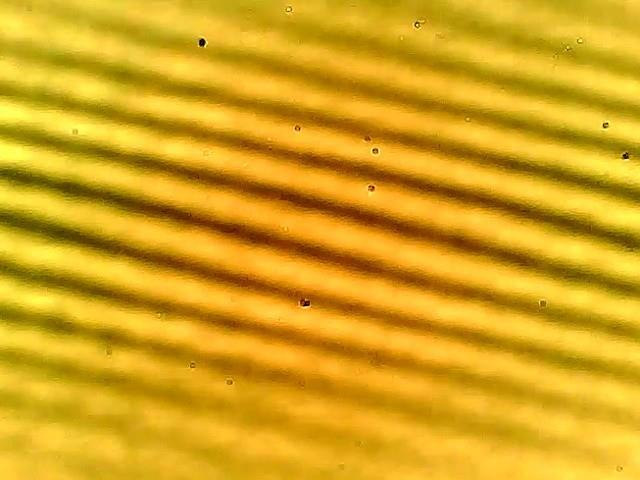
\includegraphics[width=0.48\textwidth]{assets/page5_img1_Image74.jpg}
    \caption{旋转毛玻璃条件下局部保留的干涉条纹}
    \label{fig:rotating_glass}
\end{figure}

当改变毛玻璃的位置时，毛玻璃散射形成的等效源面及其经过透镜后的成像关系发生改变，CCD 上参与干涉的两束光所对应的源面点距离也随之变化。由式~\eqref{eq:coherence} 可知，相干度对横向距离非常敏感，因此条纹出现区域会随毛玻璃位置改变而改变。

\section{思考题}
\textbf{毛玻璃位于不同位置时为什么条纹出现区域有变化？}

毛玻璃的位置改变了部分相干光源的等效源面位置、光束的会聚或发散状态以及光场横向相干尺度在干涉区域中的映射关系。由于柱透镜和反射镜使两束干涉光互为镜像，CCD 上不同位置处叠加的两束光对应于源面上不同横向间距的一对点。毛玻璃移动后，这一对应关系发生变化，满足较小横向间距、相干性较好的区域随之改变，因此能观察到明显条纹的区域也会发生变化。

\end{document}
